% tikzpic.tex
\documentclass[crop,tikz]{standalone}% 'crop' is the default for v1.0, before it was 'preview'

\usetikzlibrary{arrows,decorations.pathmorphing,decorations.pathreplacing,backgrounds,positioning,fit,matrix}
\usetikzlibrary{shapes,calc,patterns,arrows.meta}
\tikzset{
	vert/.style={circle,inner sep=1.5,fill=white,draw,minimum size=.3cm},
	edge/.style={color=black, thick},
	diredge/.style={->,>={Stealth[width=8pt,length=8pt]},color=black, thick},
	timelabel/.style={fill=white,font=\footnotesize, text centered},
	wave/.style={decorate,decoration={coil,aspect=0}},
	dirwave/.style={->, >={Stealth[width=8pt,length=8pt]},decorate,decoration={coil,aspect=0}},
	diredge2/.style={->,>={Stealth[width=8pt,length=8pt]}}
}
\begin{document}

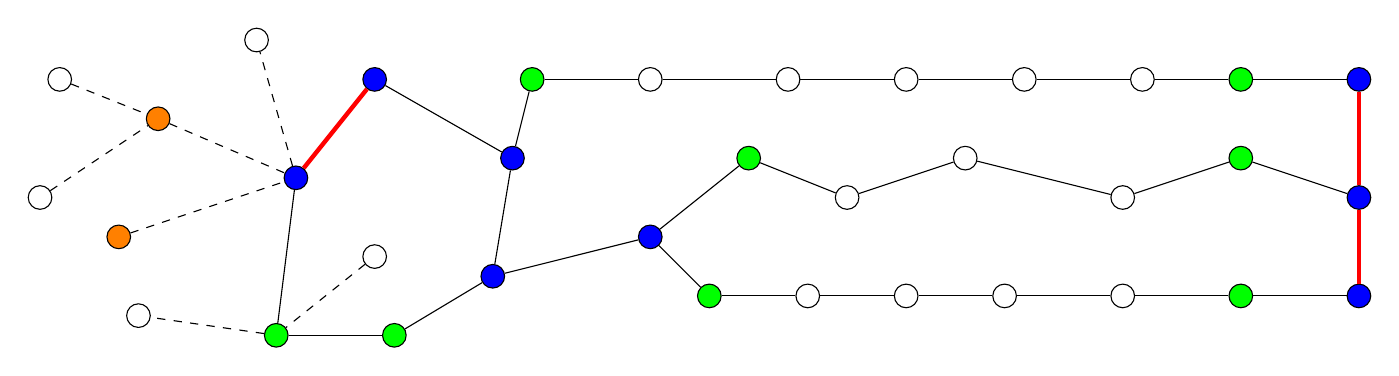
\begin{tikzpicture}
		\node [vert, fill = orange] (0) at (-9.25, 12.5) {};
		\node [vert, fill = blue] (1) at (-7, 13.25) {};
		\node [vert, fill = blue] (2) at (-6, 14.5) {};
		\node [vert, fill = blue] (3) at (-4.25, 13.5) {};
		\node [vert, fill = white] (4) at (-9, 11.5) {};
		\node [vert, fill = green] (5) at (-7.25, 11.25) {};
		\node [vert, fill = blue] (6) at (-4.5, 12) {};
		\node [vert, fill = green] (7) at (-5.75, 11.25) {};
		\node [vert, fill = blue] (8) at (-2.5, 12.5) {};
		\node [vert, fill = white] (9) at (-10.25, 13) {};
		\node [vert, fill = white] (10) at (-7.5, 15) {};
		\node [vert, fill = white] (11) at (-6, 12.25) {};
		\node [vert, fill = green] (13) at (5, 13.5) {};
		\node [vert, fill = blue] (14) at (6.5, 14.5) {};
		\node [vert, fill = orange] (16) at (-8.75, 14) {};
		\node [vert, fill = white] (17) at (-10, 14.5) {};
		\node [vert, fill = green] (19) at (5, 11.75) {};
		\node [vert, fill = blue] (20) at (6.5, 11.75) {};
		\node [vert, fill = blue] (21) at (6.5, 13) {};
		\node [vert, fill = green] (22) at (-4, 14.5) {};
		\node [vert, fill = white] (23) at (-2.5, 14.5) {};
		\node [vert, fill = white] (24) at (-0.75, 14.5) {};
		\node [vert, fill = white] (25) at (0.75, 14.5) {};
		\node [vert, fill = white] (26) at (2.25, 14.5) {};
		\node [vert, fill = white] (27) at (3.75, 14.5) {};
		\node [vert, fill = green] (28) at (5, 14.5) {};
		\node [vert, fill = green] (29) at (-1.75, 11.75) {};
		\node [vert, fill = white] (30) at (-0.5, 11.75) {};
		\node [vert, fill = white] (31) at (0.75, 11.75) {};
		\node [vert, fill = white] (32) at (2, 11.75) {};
		\node [vert, fill = white] (33) at (3.5, 11.75) {};
		\node [vert, fill = white] (34) at (3.5, 13) {};
		\node [vert, fill = white] (35) at (1.5, 13.5) {};
		\node [vert, fill = white] (36) at (0, 13) {};
		\node [vert, fill = green] (37) at (-1.25, 13.5) {};

		\draw [dashed] (0) to (1);
		\draw [dashed] (1) to (10);
		\draw (2) to (3);
		\draw (3) to (6);
		\draw (6) to (7);
		\draw (7) to (5);
		\draw [dashed] (5) to (4);
		\draw [dashed] (11) to (5);
		\draw (8) to (6);
		\draw (1) to (5);
		\draw [dashed] (17) to (16);
		\draw [dashed] (16) to (1);
		\draw (19) to (20);
		\draw (13) to (21);
		\draw [dashed] (9) to (16);
		\draw [ultra thick, red] (21) to (20);
		\draw [ultra thick, red] (14) to (21);
		\draw (22) to (23);
		\draw (23) to (24);
		\draw (24) to (25);
		\draw (25) to (26);
		\draw (26) to (27);
		\draw (27) to (28);
		\draw (28) to (14);
		\draw (3) to (22);
		\draw (8) to (29);
		\draw (29) to (30);
		\draw (30) to (31);
		\draw (31) to (32);
		\draw (32) to (33);
		\draw (33) to (19);
		\draw (13) to (34);
		\draw (34) to (35);
		\draw (35) to (36);
		\draw (36) to (37);
		\draw (37) to (8);
		\draw [ultra thick, red] (1) to (2);
\end{tikzpicture}


\end{document}